% ============================================================
%  ALP at FCC-ee Z-pole: projected constraints
%  Author: Iñaki Pardo
%  Draft — P6 Project Period 2025/2026
% ============================================================
\documentclass[12pt,a4paper]{article}

\usepackage[margin=2.5cm]{geometry}
\usepackage{amsmath,amssymb,amsfonts}
\usepackage{graphicx}
\usepackage{hyperref}
\usepackage{xcolor}
\usepackage{booktabs}
\usepackage{siunitx}
\usepackage{caption}
\usepackage{subcaption}
\usepackage[numbers,sort&compress]{natbib}
\usepackage{lineno}
\usepackage{setspace}

\onehalfspacing
\linenumbers

% ---- convenience macros ----
\newcommand{\alp}{a}
\newcommand{\gagg}{g_{a\gamma\gamma}}
\newcommand{\ma}{m_a}
\newcommand{\Lint}{\mathcal{L}}
\newcommand{\sqrts}{\sqrt{s}}
\newcommand{\MeV}{\,\text{MeV}}
\newcommand{\GeV}{\,\text{GeV}}
\newcommand{\TeV}{\,\text{TeV}}
\newcommand{\abinv}{\,\text{ab}^{-1}}
\newcommand{\pbinv}{\,\text{pb}^{-1}}
\newcommand{\dchi}{\Delta\chi^2}

\hypersetup{colorlinks=true,linkcolor=blue,citecolor=blue,urlcolor=blue}

% ============================================================
\begin{document}

\title{\textbf{Searching for Axion-Like Particles at FCC-ee:\\
    Projected Sensitivity in the Invisible and Prompt-Resolved Channels\\
    at the Z Pole}}

\author{Iñaki Pardo\\
    \small Maastricht Science Programme, Maastricht University\\
    \small \texttt{inaxpardo0204@gmail.com}}

\date{June 2026 — Project Period Draft}
\maketitle

% ============================================================
\begin{abstract}
We present projected sensitivity estimates for the production of axion-like
particles (ALPs) at the proposed Future Circular Collider operating at the
Z~pole ($\sqrts = 91.2\GeV$, $\Lint = 150\abinv$) via the associated
production process $e^+e^- \to \gamma\,\alp$.
Two detector signatures are analysed: the \emph{invisible} channel, in which
the ALP escapes the detector ($\ell_\alp > L_\mathrm{max}$), and the
\emph{prompt-resolved} channel, in which the ALP decays to two separated
photons inside the tracker ($\ell_\alp < L_\mathrm{min}$,
$\Delta\theta > \Delta\theta_\mathrm{res}$).
Signal events are generated with \textsc{MadGraph5\_{aMC@NLO}}, processed
through \textsc{Pythia\,8} for ALP decay and lifetime, and passed through
a \textsc{Delphes} fast simulation of the IDEA detector concept.
SM backgrounds for both channels are simulated, binned, and normalised to the
full target luminosity.
Projected 90\% CL exclusion contours are derived using a binned
Asimov $\dchi$ method, with analytic production and lifetime formulae corrected
by detector-level signal scans.
For the invisible channel, the analysis reaches
$\gagg \approx 5.5\times10^{-7}\GeV^{-1}$ over the ALP mass range
$0.01\text{--}0.92\GeV$.
The prompt-resolved channel extends sensitivity to
$\gagg \sim 10^{-5}\text{--}3\times10^{-4}\GeV^{-1}$ for
$m_\alp \in [0.61, 80]\GeV$.
Both projected contours surpass current collider bounds by one to two orders
of magnitude in coupling at comparable masses.
The analysis machinery is validated against the published Belle~II
ALP exclusion boundary, reproducing it to within
$|\log_{10}(g_\mathrm{closure}/g_\mathrm{published})| \leq 7.6\times10^{-3}$.
Additional validation gates check the MadGraph cross section, the ALP width and
Pythia lifetime convention, the Delphes output, and the reconstructed ALP
invariant-mass or recoil-energy observable at every detector-level signal point.
\end{abstract}

% ============================================================
\section{Introduction}
\label{sec:intro}

The Peccei--Quinn (PQ) mechanism, proposed to explain the absence of
strong CP violation~\cite{Peccei1977,Weinberg1978,Wilczek1978}, predicts the
existence of a pseudo-Nambu--Goldstone boson, the axion.
The simplest requirement for the PQ mechanism to resolve the strong CP problem
constrains the axion mass and its couplings to a narrow band in the coupling--mass
plane---the so-called QCD axion line.
However, extensions of this framework that decouple the mass from the
coupling give rise to \emph{axion-like particles} (ALPs): pseudo-scalars that
couple to Standard Model (SM) particles with arbitrary mass--coupling
combinations~\cite{Jaeckel2010,Brivio2017,Dolan2017}.

The ALP--photon coupling,
\begin{equation}
    \mathcal{L} \supset -\frac{1}{4}\gagg\,\alp\,F_{\mu\nu}\tilde{F}^{\mu\nu},
    \label{eq:lagrangian}
\end{equation}
is particularly well-motivated.
It arises generically from the anomalous coupling of any axion-like field to
the electromagnetic field strength $F_{\mu\nu}$, and is bounded across many
orders of magnitude in mass by astrophysical, cosmological, and laboratory
experiments~\cite{AxionLimits}.
In the mass range $10\MeV$--$80\GeV$ relevant to collider searches,
the most stringent direct constraints come from $e^+e^-$ collider experiments
(LEP, Belle~II, BaBar, BESIII) and beam-dump experiments, and leave significant
regions of parameter space unexplored at couplings
$\gagg \lesssim 10^{-4}\GeV^{-1}$.

The Future Circular Collider (FCC-ee) is a proposed $e^+e^-$ machine
that would operate at several centre-of-mass energies from the Z pole
($\sqrts \approx 91.2\GeV$) up to the $t\bar{t}$ threshold~\cite{FCCee_CDR,FCC_Physics}.
At the Z pole, the baseline luminosity target of $150\abinv$---corresponding
to approximately $5\times10^{12}$ Z bosons---provides an extraordinarily
clean and prolific environment for precision measurements and rare-process
searches.
For photophilic ALPs, the associated production cross section
$\sigma(e^+e^-\to\gamma\,\alp) \propto \gagg^2(1-\ma^2/s)^3$ grows quadratically with the
coupling and benefits enormously from the high luminosity, making FCC-ee a
uniquely powerful probe.
The Z-pole run is chosen as the baseline deliverable for three practical and
physics reasons. First, it is the FCC-ee stage with the largest expected
integrated luminosity, so it gives the strongest statistics-driven reach for
the single-coupling process studied here. Second, the fixed centre-of-mass
energy gives a simple mono-energetic recoil photon,
$E_\gamma=(s-\ma^2)/(2\sqrts)$, making the invisible and prompt-resolved
analyses especially transparent. Third, the Z-pole overlaps the mass range
where existing collider constraints from Belle~II, BaBar, BESIII, LEP, and the
LHC leave open regions that can be tested in a clean $e^+e^-$ environment.
Other FCC-ee stages are scientifically interesting, but each stage has a
different luminosity, background composition, recoil-energy range, and
detector acceptance optimisation. They are therefore treated as extensions
rather than part of the controlled final deliverable.

This paper presents projected ALP sensitivity estimates at the FCC-ee
Z~pole, focusing on the two experimentally cleanest signatures: the
invisible channel (ALP escapes) and the prompt-resolved channel (ALP decays
to two separated photons).
The analysis uses a complete simulation chain from matrix-element
generation to fast detector response, validated against published experimental
results.

\paragraph{Paper structure.}
Section~\ref{sec:theory} reviews the relevant ALP physics.
Section~\ref{sec:simulation} describes the simulation and detector modelling.
Section~\ref{sec:analysis} presents the signal classification, background
estimation, and limit-setting method.
Section~\ref{sec:results} reports the projected exclusion contours.
Section~\ref{sec:discussion} discusses the physics reach, limitations, and outlook.

% ============================================================
\section{Theory}
\label{sec:theory}

\subsection{Analytic model for photophilic ALPs}

This analysis assumes a single effective operator,
Eq.~\eqref{eq:lagrangian}, with all direct ALP couplings to fermions, gluons,
$W$ bosons, and $Z$ bosons set to zero at tree level. The only model
parameters scanned are therefore the ALP mass $\ma$ and the photon coupling
$\gagg$. In this benchmark the total width is taken to be
\begin{equation}
    \Gamma_\mathrm{tot} \simeq \Gamma(a\to\gamma\gamma),
    \label{eq:width_assumption}
\end{equation}
because $a\to\gamma\gamma$ is the only open tree-level decay channel in the
implemented model. Loop-induced fermion modes are neglected consistently with
the photophilic benchmark and with the UFO parameter choice used in the
simulation.

\subsection{ALP--photon vertex and associated production}

The collider event is easiest to read in the same order as it happens. First,
the incoming electron and positron annihilate through the ordinary QED vertex
into a virtual photon,
\begin{equation}
    e^+e^- \to \gamma^\ast(q),
\end{equation}
where $q=p_{e^-}+p_{e^+}$ is the four-momentum carried by the virtual photon.
This photon is \emph{off shell}: a real photon must satisfy $q^2=0$, but here
$q^2=s$, the squared centre-of-mass energy of the collision. The virtual
photon then uses the ALP--photon interaction to produce a real recoil photon
and an ALP,
\begin{equation}
    \gamma^\ast(q)\to \gamma(k)\,a(p_a).
\end{equation}
The full associated-production process is therefore
\begin{equation}
    e^+ e^- \to \gamma\,\alp,
    \label{eq:production}
\end{equation}
with the real photon providing the mono-energetic recoil tag.
Photon-fusion production
$e^+e^-\to e^+e^-a$ can have a larger inclusive rate, but it places the
scattered electrons in the forward beampipe region and is much harder to
separate from radiative Bhabha and beam-induced backgrounds. The analytic and
Monte Carlo pipeline therefore targets the recoil-photon topology.

The same ALP--photon vertex controls both this production process and the later
ALP decay. Using
\begin{equation}
    \tilde F^{\mu\nu}
    = \frac{1}{2}\epsilon^{\mu\nu\rho\sigma}F_{\rho\sigma},
    \qquad
    \epsilon^{0123}=+1,
\end{equation}
the interaction term gives the two-photon vertex
\begin{equation}
    V^{\mu\nu}(k_1,k_2)
    =
    -i\,\gagg\,
    \epsilon^{\mu\nu\alpha\beta}k_{1\alpha}k_{2\beta},
    \label{eq:vertex}
\end{equation}
where both photon momenta are taken incoming to the vertex. Here
$F_{\mu\nu}$ is the electromagnetic field-strength tensor, while
$\tilde F^{\mu\nu}$ is its dual. The object
$\epsilon^{\mu\nu\rho\sigma}$ is the four-dimensional Levi-Civita symbol:
it is completely antisymmetric, equals $+1$ for the ordered indices
$(0,1,2,3)$, changes sign whenever two indices are exchanged, and vanishes
whenever two indices are the same. Its appearance encodes the pseudoscalar,
CP-odd nature of the ALP--photon interaction. The Greek indices
$\mu,\nu,\alpha,\beta$ are Lorentz indices, and repeated indices are summed
over according to the Einstein convention. The vectors $k_1$ and $k_2$ are
the four-momenta of the two photon legs attached to the vertex. In production
one of those photon legs is the off-shell $\gamma^\ast(q)$ and the other is the
real recoil photon $\gamma(k)$.

The Born-level amplitude for Eq.~\eqref{eq:production} is
\begin{equation}
    \mathcal{M}
    =
    \frac{e\gagg}{s}
    \left[
      \bar v(p_{e^+})\gamma^\mu u(p_{e^-})
    \right]
    \epsilon_{\mu\nu\alpha\beta}
    q^\alpha k^\beta
    \varepsilon^{*\nu}(k).
    \label{eq:prod_amp}
\end{equation}
The factors in this expression have direct diagrammatic meanings. The electric
charge $e$ comes from the ordinary QED vertex where the electron--positron pair
annihilates into a virtual photon. The spinors $u(p_{e^-})$ and
$\bar v(p_{e^+})$ describe the incoming electron and positron, and
$\gamma^\mu$ is a Dirac matrix. The factor $1/s$ is the propagator of the
intermediate virtual photon after contracting with the photon-current indices.
The factor $\gagg\epsilon_{\mu\nu\alpha\beta}q^\alpha k^\beta$ is the
ALP--photon vertex from Eq.~\eqref{eq:vertex}; $q$ is the virtual-photon
momentum and $k$ is the outgoing real-photon momentum. Finally,
$\varepsilon^{*\nu}(k)$ is the polarization vector of the observed outgoing
photon.

\subsection{Two-body production kinematics and cross section}

In the centre-of-mass frame the total four-momentum is
$P^\mu=p_{e^-}^\mu+p_{e^+}^\mu=(\sqrts,0,0,0)$.
Momentum conservation gives $P^\mu=p_a^\mu+k^\mu$, with $k^2=0$ for the recoil
photon and $p_a^2=\ma^2$ for the ALP. Squaring $P-k=p_a$ gives
\begin{equation}
    (P-k)^2=\ma^2
    \quad\Rightarrow\quad
    s-2P\cdot k=\ma^2.
\end{equation}
Here $p_{e^-}$ and $p_{e^+}$ are the incoming electron and positron
four-momenta, $p_a$ is the outgoing ALP four-momentum, and $k$ is the outgoing
recoil-photon four-momentum. The invariant
$s=P^2=(p_{e^-}+p_{e^+})^2$ is the squared centre-of-mass energy, so
$\sqrts$ is the total collision energy. Since $P\cdot k=\sqrts\,E_\gamma$ in
the centre-of-mass frame, the recoil photon energy is fixed:
\begin{equation}
    E_{\gamma,\mathrm{recoil}}
    =
    \frac{s-\ma^2}{2\sqrts}.
    \label{eq:Egamma}
\end{equation}
The ALP energy and common three-momentum magnitude are therefore
\begin{equation}
    E_a
    =
    \sqrts-E_\gamma
    =
    \frac{s+\ma^2}{2\sqrts},
    \qquad
    |\mathbf{p}_a|
    =
    |\mathbf{k}|
    =
    \frac{s-\ma^2}{2\sqrts}.
    \label{eq:two_body_kinematics}
\end{equation}
These relations are the source of the mono-energetic recoil-photon signature.
They are purely kinematic: at fixed $\sqrts$ and $\ma$, a two-body final state
has no freedom to choose a different recoil-photon energy before detector
smearing or initial-state radiation. They also give the ALP boost,
\begin{equation}
    \gamma_a=\frac{E_a}{\ma},
    \qquad
    \beta_a\gamma_a=\frac{|\mathbf{p}_a|}{\ma}.
    \label{eq:boost}
\end{equation}

Averaging over the two electron and two positron spin states and summing over
the final photon polarisation gives, in the limit $m_e^2\ll s$,
\begin{equation}
    \overline{|\mathcal{M}|^2}
    =
    \frac{e^2\gagg^2s}{4}
    \left(1+\cos^2\theta_\mathrm{CM}\right)
    \left(1-\frac{\ma^2}{s}\right)^2,
    \label{eq:prod_m2}
\end{equation}
where $\theta_\mathrm{CM}$ is the recoil-photon polar angle relative to the
incoming electron direction. The spin average appears because the FCC-ee beams
are treated as unpolarized: the calculation averages over the four possible
initial spin configurations and sums over the unobserved final photon
polarization. The factor $(1+\cos^2\theta_\mathrm{CM})$ gives the angular
shape, while $(1-\ma^2/s)^2$ reflects the momentum dependence of the
pseudoscalar vertex.

The two-body phase-space formula for unpolarised $2\to2$ scattering is
\begin{equation}
    \frac{d\sigma}{d\Omega}
    =
    \frac{1}{64\pi^2s}
    \frac{|\mathbf{p}_f|}{|\mathbf{p}_i|}
    \overline{|\mathcal{M}|^2},
    \label{eq:two_body_xsec}
\end{equation}
with $|\mathbf{p}_i|=\sqrts/2$ and
$|\mathbf{p}_f|=(s-\ma^2)/(2\sqrts)$. In this expression $d\Omega$ is the
solid-angle element of the outgoing photon, $|\mathbf{p}_i|$ is the magnitude
of the incoming electron or positron three-momentum in the centre-of-mass
frame, and $|\mathbf{p}_f|$ is the magnitude of either final-state momentum.
The ratio $|\mathbf{p}_f|/|\mathbf{p}_i|$ is the two-body phase-space
suppression: if $\ma$ approaches $\sqrts$, there is little momentum left for
the final state. Integrating over the azimuthal angle then gives
\begin{equation}
    \frac{d\sigma}{d\cos\theta_\mathrm{CM}}
    =
    \frac{\alpha\,\gagg^2}{32}
    \left(1+\cos^2\theta_\mathrm{CM}\right)
    \left(1-\frac{\ma^2}{s}\right)^3.
    \label{eq:dsigma_dcostheta}
\end{equation}
The third power of $(1-\ma^2/s)$ has a useful interpretation: one power comes
from the available two-body phase space and two powers come from the
pseudoscalar momentum dependence of the $a\gamma\gamma$ vertex. Finally,
\begin{equation}
    \int_{-1}^{1}
    \left(1+\cos^2\theta\right)d\cos\theta
    =
    \frac{8}{3},
\end{equation}
so the total cross section over the full angular range is
\begin{equation}
    \sigma(e^+e^-\to\gamma\,\alp)
    =
    \frac{\alpha\,\gagg^2}{12}
    \left(1 - \frac{\ma^2}{s}\right)^3.
    \label{eq:xsec}
\end{equation}
At $\sqrts = 91.2\GeV$ and $\gagg = 10^{-3}\GeV^{-1}$,
Eq.~\eqref{eq:xsec} gives $\sigma \approx 5.5\times10^{-5}\,\text{pb}$;
at $\gagg = 10^{-6}\GeV^{-1}$ it falls to
$5.5\times10^{-11}\,\text{pb}$. The enormous FCC-ee Z-pole luminosity
($150\abinv = 1.5\times10^{8}\pbinv$) compensates for small couplings and is
what makes sensitivity below $10^{-6}\GeV^{-1}$ possible.

\subsection{ALP decay to two photons}

After the ALP is produced, it can decay through the same
$a\gamma\gamma$ vertex into two photons,
\begin{equation}
    a(p)\to\gamma(k_1)\gamma(k_2).
\end{equation}
The decay amplitude is
\begin{equation}
    \mathcal{M}
    =
    -\gagg\,
    \epsilon^{\mu\nu\alpha\beta}
    k_{1\alpha}k_{2\beta}
    \varepsilon^{*}_{1\mu}\varepsilon^{*}_{2\nu}.
    \label{eq:decay_amp}
\end{equation}
In this equation $p$ is the ALP four-momentum, while
$k_1$ and $k_2$ are the four-momenta of the two decay photons.
$\varepsilon_{1\mu}$ and $\varepsilon_{2\nu}$ are the photon polarization
four-vectors. The star means complex conjugation, as appropriate for outgoing
external particles. These polarization vectors describe the two physical
transverse polarization states of a photon. They should not be confused with
the Levi-Civita symbol $\epsilon^{\mu\nu\alpha\beta}$; the different symbol
$\varepsilon^\mu$ is used here to keep the two concepts separate.

The detector does not measure the photon polarization in this analysis.
Therefore the observable decay probability must include all allowed final
polarization states. This is why we compute
$\sum_\mathrm{pol}|\mathcal{M}|^2$ rather than a single fixed-polarization
amplitude. Because the amplitude is gauge invariant, terms proportional to a
photon momentum vanish by the Ward identity, so the physical polarization sums
can be replaced by the compact covariant expression
$\sum_\lambda \varepsilon_\mu^{(\lambda)*}
\varepsilon_{\mu'}^{(\lambda)}\to -g_{\mu\mu'}$. With the mostly-minus metric,
this gives
\begin{align}
    \sum_\mathrm{pol}|\mathcal{M}|^2
    &=
    \gagg^2\,
    \epsilon^{\mu\nu\alpha\beta}
    \epsilon_{\mu\nu}^{\phantom{\mu\nu}\alpha'\beta'}
    k_{1\alpha}k_{2\beta}k_{1\alpha'}k_{2\beta'} \nonumber\\
    &=
    -2\gagg^2
    \left[
      k_1^2 k_2^2 - (k_1\cdot k_2)^2
    \right].
    \label{eq:decay_m2_step}
\end{align}
The first line follows from multiplying Eq.~\eqref{eq:decay_amp} by its complex
conjugate and summing over the two photon polarizations. The second line uses
the standard Levi-Civita contraction identity
\begin{equation}
    \epsilon^{\mu\nu\alpha\beta}
    \epsilon_{\mu\nu}^{\phantom{\mu\nu}\alpha'\beta'}
    =
    -2\left(
      g^{\alpha\alpha'}g^{\beta\beta'}
      -
      g^{\alpha\beta'}g^{\beta\alpha'}
    \right).
    \label{eq:levicivita_contraction}
\end{equation}
The photons are on shell and massless, so $k_1^2=k_2^2=0$. Momentum
conservation gives $p=k_1+k_2$, and because the ALP is on shell,
$p^2=\ma^2$. Therefore
$\ma^2=(k_1+k_2)^2=2k_1\cdot k_2$, so
\begin{equation}
    \sum_\mathrm{pol}|\mathcal{M}|^2
    =
    2\gagg^2(k_1\cdot k_2)^2
    =
    \frac{\gagg^2\ma^4}{2}.
    \label{eq:decay_m2}
\end{equation}

For correctly paired photons from the ALP decay,
\begin{equation}
    M_{\gamma\gamma}^2=(k_1+k_2)^2
    =
    2E_1E_2(1-\cos\theta_{12})
    =
    \ma^2.
    \label{eq:mgg}
\end{equation}
Here $E_1$ and $E_2$ are the measured photon energies and $\theta_{12}$ is the
opening angle between the two photons. This invariant mass is independent of
the lab-frame boost of the ALP, so correctly paired decay photons form a peak
at $M_{\gamma\gamma}=\ma$. That peak is the analysis observable in the
prompt-resolved channel.

For a two-body decay into identical massless particles,
\begin{equation}
    \Gamma
    =
    \frac{1}{2\ma}\frac{1}{2!}
    \int d\Phi_2\,\sum_\mathrm{pol}|\mathcal{M}|^2,
    \qquad
    \int d\Phi_2 = \frac{1}{8\pi}.
    \label{eq:decay_phase_space}
\end{equation}
This formula is Fermi's golden rule written in relativistic form. The factor
$1/(2\ma)$ is the flux normalization for one decaying particle of mass $\ma$.
The factor $1/2!$ is essential because the two final photons are identical:
without it, the same physical final state would be counted twice when the
labels $1$ and $2$ are exchanged. The object $d\Phi_2$ is the Lorentz-invariant
two-body phase-space element; for two massless particles integrated over all
directions it equals $1/(8\pi)$. Equivalently,
$\Gamma=(1/2!)\,|\mathbf{k}|\,|\mathcal{M}|^2/(8\pi \ma^2)$ with
$|\mathbf{k}|=\ma/2$, where $|\mathbf{k}|$ is the magnitude of either photon
three-momentum in the ALP rest frame. Substituting Eq.~\eqref{eq:decay_m2}
gives the width used throughout the project:
\begin{equation}
    \Gamma(\alp\to\gamma\gamma)
    =
    \frac{\gagg^2\,\ma^3}{64\pi}.
    \label{eq:width}
\end{equation}

The proper lifetime and proper decay length are then
\begin{equation}
    \tau_a=\frac{1}{\Gamma_a},
    \qquad
    c\tau_a=\frac{\hbar c}{\Gamma_a},
    \label{eq:proper_lifetime}
\end{equation}
with $\hbar c=1.973269804\times10^{-16}\,\GeV\,\mathrm{m}$. The lifetime
$\tau_a$ is the mean time before decay in the ALP rest frame. Multiplying by
$c$ converts this time into the mean proper distance travelled in that rest
frame. In the lab frame the decay length is increased by the boost,
\begin{equation}
    \ell_\alp
    =
    \beta_a\gamma_a c\tau_a
    =
    \frac{|\mathbf{p}_a|}{\ma}
    \frac{\hbar c}{\Gamma(a\to\gamma\gamma)}.
    \label{eq:lifetime}
\end{equation}
where $\beta_a=v_a/c$, $\gamma_a=E_a/\ma$, and
$\beta_a\gamma_a=|\mathbf{p}_a|/\ma$. This is the quantity that determines
whether the ALP decays before the tracker, inside the detector, or outside the
calorimeter.
Equations~\eqref{eq:width} and~\eqref{eq:lifetime} show that $\ell_\alp$
decreases with increasing $\gagg$ and increasing $\ma$:
heavy, strongly coupled ALPs decay promptly, while light, weakly coupled ALPs
are long-lived and escape the detector.

\subsection{Decay probabilities and photon separation}

The probability density for an ALP to decay after travelling a lab-frame
distance $L$ is exponential,
\begin{equation}
    f(L)=\frac{1}{\ell_a}e^{-L/\ell_a}.
\end{equation}
This is the usual decay law written in distance rather than time. The parameter
$\ell_a$ is the mean lab-frame decay distance from Eq.~\eqref{eq:lifetime}; a
larger $\ell_a$ means that the ALP is more likely to survive to the calorimeter
or escape the detector. Integrating this density over the relevant detector
length intervals gives the probabilities used in the analytic scan:
\begin{align}
    P(L>L_\mathrm{max})
    &=
    e^{-L_\mathrm{max}/\ell_a},
    \label{eq:survival_prob}\\
    P(L<L_\mathrm{min})
    &=
    1-e^{-L_\mathrm{min}/\ell_a},\\
    P(L_\mathrm{min}<L<L_\mathrm{max})
    &=
    e^{-L_\mathrm{min}/\ell_a}
    -
    e^{-L_\mathrm{max}/\ell_a}.
    \label{eq:decay_window_prob}
\end{align}
The first line is the survival probability to the outer detector radius
$L_\mathrm{max}$ and defines the invisible signature. The second is the
probability to decay before the prompt-distance scale $L_\mathrm{min}$. The
third is the probability to decay between those two scales, producing a
displaced signature. These probabilities define the invisible, prompt, and
displaced regions of the grid.

The angular resolution boundary follows from boosting the isotropic
$a\to\gamma\gamma$ decay. For an ALP moving along the $z$ axis, the two photons
are emitted back-to-back in the ALP rest frame. The smallest lab-frame opening
angle occurs when the rest-frame photons are emitted transverse to the boost,
for which
\begin{equation}
    \Delta\theta_{\gamma\gamma}^{\min}
    =
    2\arctan\!\left(\frac{1}{\gamma_a\beta_a}\right)
    =
    2\arctan\!\left(\frac{\ma}{|\mathbf{p}_a|}\right).
    \label{eq:dtheta_exact}
\end{equation}
The physical reason is simple: a highly boosted ALP carries the two decay
photons forward in almost the same direction, so the two electromagnetic
showers can merge in the calorimeter. Equation~\eqref{eq:dtheta_exact} uses the
exact boost factor through $\gamma_a\beta_a=|\mathbf{p}_a|/\ma$.
For light ALPs, $|\mathbf{p}_a|\simeq\sqrts/2$ and
$\gamma_a\simeq\sqrts/(2\ma)$, so
\begin{equation}
    \Delta\theta_{\gamma\gamma}^{\min}
    \simeq
    \frac{2}{\gamma_a}
    \simeq
    \frac{4\ma}{\sqrts}.
    \label{eq:dtheta}
\end{equation}
The prompt-resolved channel requires this opening angle to be larger than the
detector angular resolution, $\Delta\theta_\mathrm{res}$. If
$\Delta\theta_{\gamma\gamma}^{\min}<\Delta\theta_\mathrm{res}$, the two photons
are treated as merged even if the ALP decays promptly.

\subsection{Signal signatures}

The ALP phenomenology at the detector level is determined by two quantities:
the decay length $\ell_\alp$ and the minimum diphoton opening angle
$\Delta\theta_\mathrm{min}$ of the ALP decay products.
The opening-angle criterion uses the boosted two-body result derived in
Eq.~\eqref{eq:dtheta}.
We classify each point $(m_\alp, \gagg)$ in the parameter space into four
exclusive signatures:

\begin{itemize}
    \item \textbf{Invisible} ($\ell_\alp > L_\mathrm{max}$):
    the ALP escapes before decaying. The signature is a single photon with
    missing energy, $e^+e^-\to\gamma + \not\!E$.

    \item \textbf{Prompt-resolved} ($\ell_\alp < L_\mathrm{min}$ and
    $\Delta\theta_\mathrm{min} \geq \Delta\theta_\mathrm{res}$):
    the ALP decays immediately to two resolvable photons,
    $e^+e^-\to\gamma\,(\to\gamma\gamma)$. The three-photon final state
    carries an invariant-mass peak at $\ma$.

    \item \textbf{Displaced-resolved} ($L_\mathrm{min} \leq \ell_\alp \leq L_\mathrm{max}$):
    the ALP decays inside the detector volume but away from the interaction point.

    \item \textbf{Merged} ($\ell_\alp \leq L_\mathrm{max}$ and
    $\Delta\theta_\mathrm{min} < \Delta\theta_\mathrm{res}$):
    the ALP decay photons are not angularly resolved; the signature resembles a
    single broad photon cluster.
\end{itemize}

The invisible and prompt-resolved signatures are the primary targets of this
analysis. Displaced and merged signatures require dedicated reconstruction and
background models, so they are classified but not included as exclusion
contours in the present study.

% ============================================================
\section{Simulation and Detector Modelling}
\label{sec:simulation}

\subsection{Signal generation and computational strategy}

Signal events are generated using \textsc{MadGraph5\_aMC@NLO}~\cite{MG5} with a
UFO model implementing the ALP effective field theory of Eq.~\eqref{eq:lagrangian}.
The dense exclusion scan is not produced by running a full detector simulation
at every point in the $180\times180$ mass--coupling grid. Instead, the code uses
a two-level strategy:
\begin{enumerate}
    \item The full $(m_a,\gagg)$ grid is evaluated analytically using
    Eqs.~\eqref{eq:xsec}--\eqref{eq:dtheta}. This gives the production cross
    section, lifetime, decay-region probability, recoil energy, and opening
    angle for each point.
    \item A finite set of contour-relevant points is passed through the full
    detector-level chain. These points are used to validate the matrix element,
    lifetime convention, Delphes output, and analysis observables, and to build
    branch-aware detector correction factors.
\end{enumerate}

This separation is possible because associated production contains one ALP
photon vertex, so at tree level
$\sigma(e^+e^-\to\gamma a)\propto\gagg^2$ exactly. The shape of the production
process is therefore controlled mainly by $m_a$ and $\sqrts$, while the coupling
rescales the yield and changes the lifetime.

\subsection{Choice of scan ranges}

The final FCC-ee projection is evaluated on a logarithmic
$180\times180$ grid,
\begin{equation}
    \ma \in [10^{-2},80]\GeV,
    \qquad
    \gagg \in [10^{-8},10^{-1}]\GeV^{-1}.
    \label{eq:scan_range}
\end{equation}
The lower mass bound, $10\MeV$, is chosen because below this value the
FCC-ee Z-pole diphoton opening angle
$\Delta\theta_\mathrm{min}\simeq4\ma/\sqrts$ is far below the conservative
IDEA angular resolution used here. For example, at $m_a=10\MeV$ the opening
angle is only $0.025^\circ$, compared with
$\Delta\theta_\mathrm{res}=1.5^\circ$. Any prompt decay would therefore be a
merged-photon object, while weakly coupled ALPs are invisible. Dedicated
merged-cluster and very-low-mass beam-dump-style treatments are outside the
scope of the current collider projection.

The upper mass bound, $80\GeV$, is set by the kinematic and practical reach of
associated production at $\sqrts=91.2\GeV$. The hard kinematic condition is
$\ma<\sqrts$, but the recoil photon energy becomes small and the
$(1-\ma^2/s)^3$ phase-space factor suppresses the cross section near the
endpoint. Stopping at $80\GeV$ retains the high-mass collider region where the
prompt-resolved channel is meaningful, while avoiding a threshold-dominated
tail where a full experimental analysis would need a different low-recoil
selection.

The coupling interval in Eq.~\eqref{eq:scan_range} is deliberately wider than
the final visible contours. Values below $10^{-8}\GeV^{-1}$ are far below the
150~ab$^{-1}$ event-yield threshold because
$\sigma\propto\gagg^2$. Values up to $10^{-1}\GeV^{-1}$ are included to ensure
that the invisible upper lifetime boundary is bracketed for the lightest
masses. This upper end should not be interpreted as an equally reliable EFT
region for every ALP model. In the UFO parameter-card writer we keep
$f_a=1000\GeV$ fixed and vary $K_B+K_W$ to realise the requested physical
$\gagg$; very large $\gagg$ therefore corresponds to large dimensionless
Wilson coefficients and is used mainly as a numerical bracket for the
lifetime transition.

The detector-level chain for one signal point is:
\begin{equation}
    \begin{aligned}
    \texttt{param\_card}
    &\to \textsc{MadGraph}\;(\text{LHE})
    \to \textsc{Pythia}\;(\text{HepMC})\\
    &\to \textsc{Delphes}\;(\text{ROOT})
    \to \text{Python validation}.
    \end{aligned}
    \label{eq:pipeline}
\end{equation}
The imported UFO does not expose $\gagg$ directly. The code writes a
point-specific parameter card by mapping the physical coupling to the UFO
parameters $f_a$, $K_B$, and $K_W$ through
\begin{equation}
    \gagg=
    \frac{\alpha_\mathrm{em}(K_B+K_W)}
    {\sqrt{2}\,\pi f_a}.
    \label{eq:ufo_mapping}
\end{equation}
The UFO also contains an $a\gamma Z$ vertex. In the imported model this vertex
is proportional to
\begin{equation}
    C_{\gamma Z} \propto K_W c_w^2 - K_B s_w^2,
    \label{eq:cgz}
\end{equation}
where $s_w$ and $c_w$ are computed from the same electroweak inputs as the UFO.
The default parameter-card writer therefore uses
\begin{equation}
    K_B = (K_B+K_W)c_w^2,
    \qquad
    K_W = (K_B+K_W)s_w^2,
    \label{eq:photophilic_split}
\end{equation}
which makes Eq.~\eqref{eq:cgz} vanish at tree level while keeping the
$a\gamma\gamma$ coupling of Eq.~\eqref{eq:ufo_mapping}. This choice is essential
for the interpretation of the project. It isolates the one-parameter
photophilic benchmark, makes the MadGraph production normalisation comparable
to Eq.~\eqref{eq:xsec} and to the Belle~II closure, and prevents the Z-pole
projection from being contaminated by resonant $Z\to\gamma a$ production.
Including a genuine ALP--Z coupling is a separate physics question with a
different operator, different rates, and different signal interpretation.

For lifetime-dependent results, the code writes the project convention
\begin{equation}
    \Gamma(a\to\gamma\gamma)=\frac{\gagg^2 m_a^3}{64\pi}
\end{equation}
directly into the \texttt{DECAY 9999} block of the parameter card. Pythia then decays
the ALP to $\gamma\gamma$ with the corresponding proper lifetime. The resulting
HepMC event record is passed to
\textsc{Delphes~3}~\cite{Delphes} for fast detector simulation using
the IDEA detector card~\cite{IDEA}.

\subsection{Repository implementation and data products}

The repository mirrors the physics pipeline. Analytic formulae and validation
gates live in the theory layer; MadGraph, Pythia, HepMC, and Delphes wrappers
live in the MC layer; background building, signal-efficiency correction,
projection solving, and plotting live in the analysis layer. The main
machine-readable inputs are the locked JSON files specifying the Belle~II
closure and FCC-ee Z-pole assumptions. The main checked-in outputs are:
\begin{itemize}
    \item the analytic theory grid;
    \item the Belle~II closure curve, plot, and JSON summary;
    \item binned FCC-ee background histograms for the resolved and invisible
    channels;
    \item the collected 284-point detector-level ALP signal summary;
    \item the branch-aware full-analysis efficiency map;
    \item the FCC-ee projection CSV and signature-classification grid;
    \item the full, close-up, and combined ALP-photon money plots.
\end{itemize}
Large raw production files such as LHE, HepMC, ROOT, and full Condor work
directories are deliberately not versioned. They are reproducible intermediate
products, while the compact CSV, JSON, PNG, and PDF outputs are the
report-facing deliverables.

\subsection{Detector modelling}

The IDEA detector concept~\cite{IDEA} is a proposed FCC-ee detector featuring
a solenoidal magnetic field, silicon tracking, a drift chamber, and a
crystal electromagnetic calorimeter.
The key detector parameters used in this analysis are:
\begin{itemize}
    \item Photon acceptance: $|\eta| < 3.0$, $E_\gamma > 0.5\GeV$;
    \item Photon reconstruction efficiency: 99\%;
    \item Diphoton angular resolution: $\Delta\theta_\mathrm{res} = 1.5^\circ$
    (conservative calorimeter-cell scale, $\pi/120$);
    \item Tracker inner radius ($L_\mathrm{min}$): $0.02\,\text{m}$;
    \item Tracker/calorimeter outer radius ($L_\mathrm{max}$): $2.5\,\text{m}$.
\end{itemize}
These values are locked in
\texttt{analysis/configs/fccee\_zpole\_inputs.json}. The final deliverable
uses the assumptions in Table~\ref{tab:locked_assumptions}; changing any of
these inputs requires regenerating the classification grid, contours, and
money plots.

\begin{table}[t]
    \centering
    \caption{Locked assumptions used for the final FCC-ee Z-pole deliverable.}
    \label{tab:locked_assumptions}
    \begin{tabular}{p{0.27\textwidth}p{0.26\textwidth}p{0.37\textwidth}}
        \toprule
        Ingredient & Value & Role in the analysis \\
        \midrule
        Collider stage &
        $\sqrts=91.2\GeV$, $\Lint=150\abinv$ &
        Baseline FCC-ee Z-pole scenario; sets recoil energy, production
        phase space, and event normalisation. \\
        Physics benchmark &
        Photophilic ALP, $C_{\gamma Z}=0$ at tree level &
        Keeps the result a one-coupling $\gagg$ projection rather than a
        mixed photon--Z benchmark. \\
        Scan domain &
        $\ma=0.01$--$80\GeV$,
        $\gagg=10^{-8}$--$10^{-1}\GeV^{-1}$ &
        Covers the FCC-ee mass reach and brackets both the lower sensitivity
        floor and upper invisible lifetime boundary. \\
        Signal regions &
        Invisible and prompt-resolved only &
        These are the two channels with simple robust observables:
        recoil-photon energy and $M_{\gamma\gamma}$. \\
        Detector lengths &
        $L_\mathrm{min}=0.02\,\text{m}$,
        $L_\mathrm{max}=2.5\,\text{m}$ &
        Define prompt, displaced, and invisible decay probabilities. \\
        Photon reconstruction &
        $|\eta|<3.0$, $E_\gamma>0.5\GeV$,
        $\epsilon_\gamma=0.99$ &
        Implements the IDEA-like photon acceptance and reconstruction
        efficiency. \\
        Angular resolution &
        $\Delta\theta_\mathrm{res}=1.5^\circ$ &
        Defines whether $a\to\gamma\gamma$ is resolved or merged. \\
        Analysis resolutions &
        $\sigma_M=\max(0.05\ma,0.05\GeV)$,
        $\sigma_E=\max(0.05E_\gamma,0.5\GeV)$ &
        Widths of the Gaussian signal templates in the resolved and invisible
        binned likelihoods. \\
        SM backgrounds &
        $e^+e^-\to\gamma\gamma\gamma$ and
        $e^+e^-\to\gamma\nu\bar{\nu}$ &
        Irreducible backgrounds for the prompt-resolved and invisible
        channels, respectively. \\
        Statistical criterion &
        One-sided 90\% CL, $\dchi=2.71$, with a 3-event floor &
        Converts binned signal-plus-background expectations into exclusion
        contours. \\
        External constraints &
        AxionLimits commit
        \texttt{7d375f4879b32406}\newline
        \texttt{a239fe48d2615a4b}\newline
        \texttt{fd9bc0bb} &
        Provides the published ALP, QCD-axion, astrophysical, cosmological,
        and laboratory landscape used only as context for the money plots. \\
        \bottomrule
    \end{tabular}
\end{table}

\subsection{Validation gates}

Before applying the analysis to FCC-ee kinematics, the pipeline is checked by a
set of validation gates. These gates are run by the repository validation
scripts and by the full signal-production wrapper. They test both the physics
formulae and the file handoff between programs.

\begin{table}[h]
    \centering
    \caption{Validation gates implemented in the analysis pipeline.}
    \label{tab:gates}
    \begin{tabular}{p{0.18\textwidth}p{0.42\textwidth}p{0.30\textwidth}}
        \toprule
        Gate & What is tested & Current status \\
        \midrule
        Software smoke test &
        A generic $e^+e^-\to\mu^+\mu^-$ chain proves that MadGraph, Pythia,
        HepMC, Delphes, ROOT, and the Python reader work together. &
        Integrated as the cluster setup test. \\
        Gate 1: cross section &
        The MadGraph integrated weight for $e^+e^-\to\gamma a$ is compared to
        Eq.~\eqref{eq:xsec} at the generated $(m_a,\gagg,\sqrts)$ point. &
        Passed for 284/284 detector-level ALP scan points. \\
        Gate 2: width and lifetime &
        The UFO width convention is checked, the project $64\pi$ width is
        written into the parameter card, and the Pythia input lifetime is
        checked against Eq.~\eqref{eq:lifetime}. &
        Convention locked to Eq.~\eqref{eq:width}; Pythia summaries are checked
        per point. \\
        Gate 3: Belle~II closure &
        The Belle~II public contour is reconstructed using the same production,
        lifetime, and prompt/resolved logic as the FCC-ee projection. &
        Passed with maximum log residual $7.6\times10^{-3}$. \\
        Detector-observable gate &
        Resolved points must reconstruct a diphoton mass near $m_a$; invisible
        points must reconstruct the recoil photon near Eq.~\eqref{eq:Egamma}. &
        Passed for 284/284 detector-level ALP scan points. \\
        Background gate &
        SM background ROOT outputs are converted to binned luminosity-normalised
        histograms used directly by the limit solver. &
        Two full-stat 10\,000-event background channels included. \\
        \bottomrule
    \end{tabular}
\end{table}

The Belle~II closure is the most important external validation anchor.
Belle~II operates at $\sqrts = 10.58\GeV$ with $445\pbinv$ and uses the same
process $e^+e^-\to\gamma\,a$, $a\to\gamma\gamma$.
The procedure infers the effective signal-yield threshold implied by the
digitised Belle~II boundary from AxionLimits~\cite{AxionLimits}. It then checks
that the project production cross section, decay width, lifetime convention,
and prompt/resolved region logic reproduce the same contour. The closure test
yields
\begin{equation}
    \max_{\ma}
    \left|\log_{10}\!\left(\frac{g_\mathrm{closure}}{g_\mathrm{published}}\right)\right|
    = 7.6\times10^{-3},
    \label{eq:closure}
\end{equation}
well within the 2\% tolerance used as the acceptance criterion.
This demonstrates that the analytic model, lifetime convention, and
signal-region logic are all internally consistent and agree with a published
experimental result.

\subsection{SM background samples}

Background events are simulated at $\sqrts = 91.2\GeV$ with
\textsc{MadGraph5\_aMC@NLO} + \textsc{Pythia~8} + \textsc{Delphes/IDEA}.
Two channels are generated:
\begin{itemize}
    \item \textbf{Resolved-prompt background}: $e^+e^-\to\gamma\gamma\gamma$
    (SM QED triple-photon production),
    with $\sigma = 7.306\,\text{pb}$ and $N_\mathrm{gen} = 10\,000$ events.

    \item \textbf{Invisible background}: $e^+e^-\to\gamma\nu\bar{\nu}$
    (radiative neutrino production),
    with $\sigma = 134.9\,\text{pb}$ and $N_\mathrm{gen} = 10\,000$ events.
\end{itemize}
Backgrounds are normalised to $\Lint = 150\abinv$.
At full luminosity, the expected number of background events across the analysis
histograms is $2.58\times10^9$ (resolved) and $5.43\times10^9$ (invisible).
The resolved background is the dominant QED irreducible process for the three-photon
topology; the invisible background is the leading electroweak process with a
photon plus missing energy.

% ============================================================
\section{Analysis}
\label{sec:analysis}

\subsection{Signature classification grid}

Each of the $180\times180 = 32\,400$ grid points $(m_\alp, \gagg)$ is
classified into one of the four signatures using the analytic formulae of
Section~\ref{sec:theory}.
With the IDEA detector assumptions, the grid decomposes as follows
(Table~\ref{tab:classification}):

\begin{table}[h]
    \centering
    \caption{Signature classification of the $(m_\alp, \gagg)$ grid.}
    \label{tab:classification}
    \begin{tabular}{lrc}
        \toprule
        Signature & Grid points & Fraction \\
        \midrule
        Prompt-resolved & 14\,171 & 43.7\% \\
        Invisible        & 10\,452 & 32.3\% \\
        Merged           &  5\,989 & 18.5\% \\
        Displaced-resolved & 1\,788 &  5.5\% \\
        \midrule
        Total & 32\,400 & 100\% \\
        \bottomrule
    \end{tabular}
\end{table}

The prompt-resolved region dominates at high $\gagg$ and intermediate $\ma$,
where the ALP decays promptly and the photons are resolvable.
The invisible region covers most of the low-coupling parameter space, where
the decay length exceeds the detector radius.
The prompt-resolved threshold mass is set by
$\Delta\theta_\mathrm{min} = \Delta\theta_\mathrm{res}$:
\begin{equation}
    m_\alp^\mathrm{thresh} = \frac{\sqrts\,\Delta\theta_\mathrm{res}}{4}
    \approx \frac{91.2\GeV \times 0.0262}{4} \approx 0.597\GeV.
    \label{eq:threshold}
\end{equation}
Below this mass, the photon pair from ALP decay would be reconstructed as a
single cluster, falling into the merged category.

\subsection{Signal efficiency and detector corrections}

The expected number of signal events for a given grid point is:
\begin{equation}
    N_\mathrm{sig} = \Lint \cdot
    \sigma(\ma, \gagg) \cdot
    P_\mathrm{region}(\ma, \gagg) \cdot
    \epsilon_\mathrm{param} \cdot
    C_\mathrm{Delphes},
    \label{eq:nsig}
\end{equation}
where $P_\mathrm{region}$ is the analytic probability that the ALP falls in the
target signature region:
\begin{align}
    P_\mathrm{invisible} &= e^{-L_\mathrm{max}/\ell_\alp},
    \label{eq:pinv}\\
    P_\mathrm{prompt} &= 1 - e^{-L_\mathrm{min}/\ell_\alp}.
    \label{eq:pprompt}
\end{align}
The parametric efficiency $\epsilon_\mathrm{param}$ accounts for angular
acceptance and photon reconstruction. For the invisible channel it is the
single-photon acceptance times one photon-efficiency factor; for the
prompt-resolved channel it is the same acceptance times three photon-efficiency
factors. The remaining detector response is absorbed into the
Delphes-derived correction factor.
The detector correction factor $C_\mathrm{Delphes}$ is derived from
a channel-aware scan of 284 signal points through the full \textsc{Delphes}
simulation.
For each point, the full analysis pipeline---including the signal observable
histogram, background comparison, and analysis bin acceptance---is compared to
the analytic expectation.
The resulting correction is interpolated as a function of ALP mass separately
for each branch.
Across the signal scan, the mean detector correction factors are:
\begin{itemize}
    \item Invisible lower branch: $\langle C \rangle = 0.998$ (range 0.969--1.003),
    \item Invisible upper branch: $\langle C \rangle = 7.8\times10^6$ (extremely large
    correction from the non-monotonic $g$ dependence of the invisible yield; this
    branch is numerically fragile),
    \item Prompt-resolved: $\langle C \rangle = 1.02$ (range 0.900--2.62).
\end{itemize}

\subsection{Limit-setting method}

A projected 90\% confidence level (CL) exclusion is derived using a
binned Asimov $\dchi$ test~\cite{Cowan2011}.
For a given mass hypothesis, the analysis observable is:
\begin{itemize}
    \item Resolved channel: the diphoton invariant mass $M_{\gamma\gamma}$,
    with the signal modelled as a Gaussian centred at $\ma$ with width
    $\sigma_M = \max(0.05\,\ma,\, 0.05\GeV)$;
    \item Invisible channel: the recoil photon energy $E_\gamma$,
    with the signal modelled as a Gaussian centred at $(s-\ma^2)/(2\sqrts)$
    with width $\sigma_E = \max(0.05\,E_\gamma,\, 0.5\GeV)$.
    The histogram uses 264 bins over $[0, 50]\GeV$, extending beyond
    the nominal $\sqrts/2 = 45.6\GeV$ endpoint to retain
    detector- and ISR-smeared signal events.
\end{itemize}

For each mass point, the minimum signal yield required for exclusion is:
\begin{equation}
    N_\mathrm{sig}^\mathrm{req} =
    \max\!\left(3,\;
    \sqrt{\frac{2.71}{\displaystyle\sum_i f_i^2 / \max(B_i, 1)}}
    \right),
    \label{eq:nsig_req}
\end{equation}
where $f_i$ is the normalised signal fraction in bin $i$, $B_i$ is the expected
SM background in that bin, and 3 is a conservative event-count floor.
The threshold $\dchi = 2.71$ corresponds to a one-sided 90\% CL.
The contour in the $(m_\alp, \gagg)$ plane is then the locus of points where
$N_\mathrm{sig}(\ma, \gagg) = N_\mathrm{sig}^\mathrm{req}(\ma)$.

Because the invisible signal yield is non-monotonic in $\gagg$---it peaks at
intermediate coupling and falls off both towards small coupling (fewer events
produced) and large coupling (ALP decays before reaching $L_\mathrm{max}$)---the
invisible contour has two branches:
the \emph{lower branch} (sensitivity floor from statistics) and the
\emph{upper branch} (sensitivity ceiling from lifetime).

% ============================================================
\section{Results}
\label{sec:results}

\subsection{Signature map}

Figure~\ref{fig:classification} shows the classification of the
$(m_\alp, \gagg)$ plane under the IDEA detector assumptions.
The four signatures occupy well-separated regions.
The invisible region (blue) dominates at low coupling over a wide mass range;
the prompt-resolved region (red) covers the high-coupling, intermediate-mass
space above the resolved threshold; the merged region (orange) occupies the
low-mass, high-coupling corner where photon pairs are not angularly resolved;
and the displaced-resolved band (green) forms a narrow transition strip.
The physics boundaries between regions---the $\ell_a = L_\mathrm{min}$ and
$\ell_a = L_\mathrm{max}$ curves computed from Eqs.~\eqref{eq:width} and
\eqref{eq:lifetime}---are overlaid as dashed lines and agree with the
classification boundaries to machine precision.

\begin{figure}[h]
    \centering
    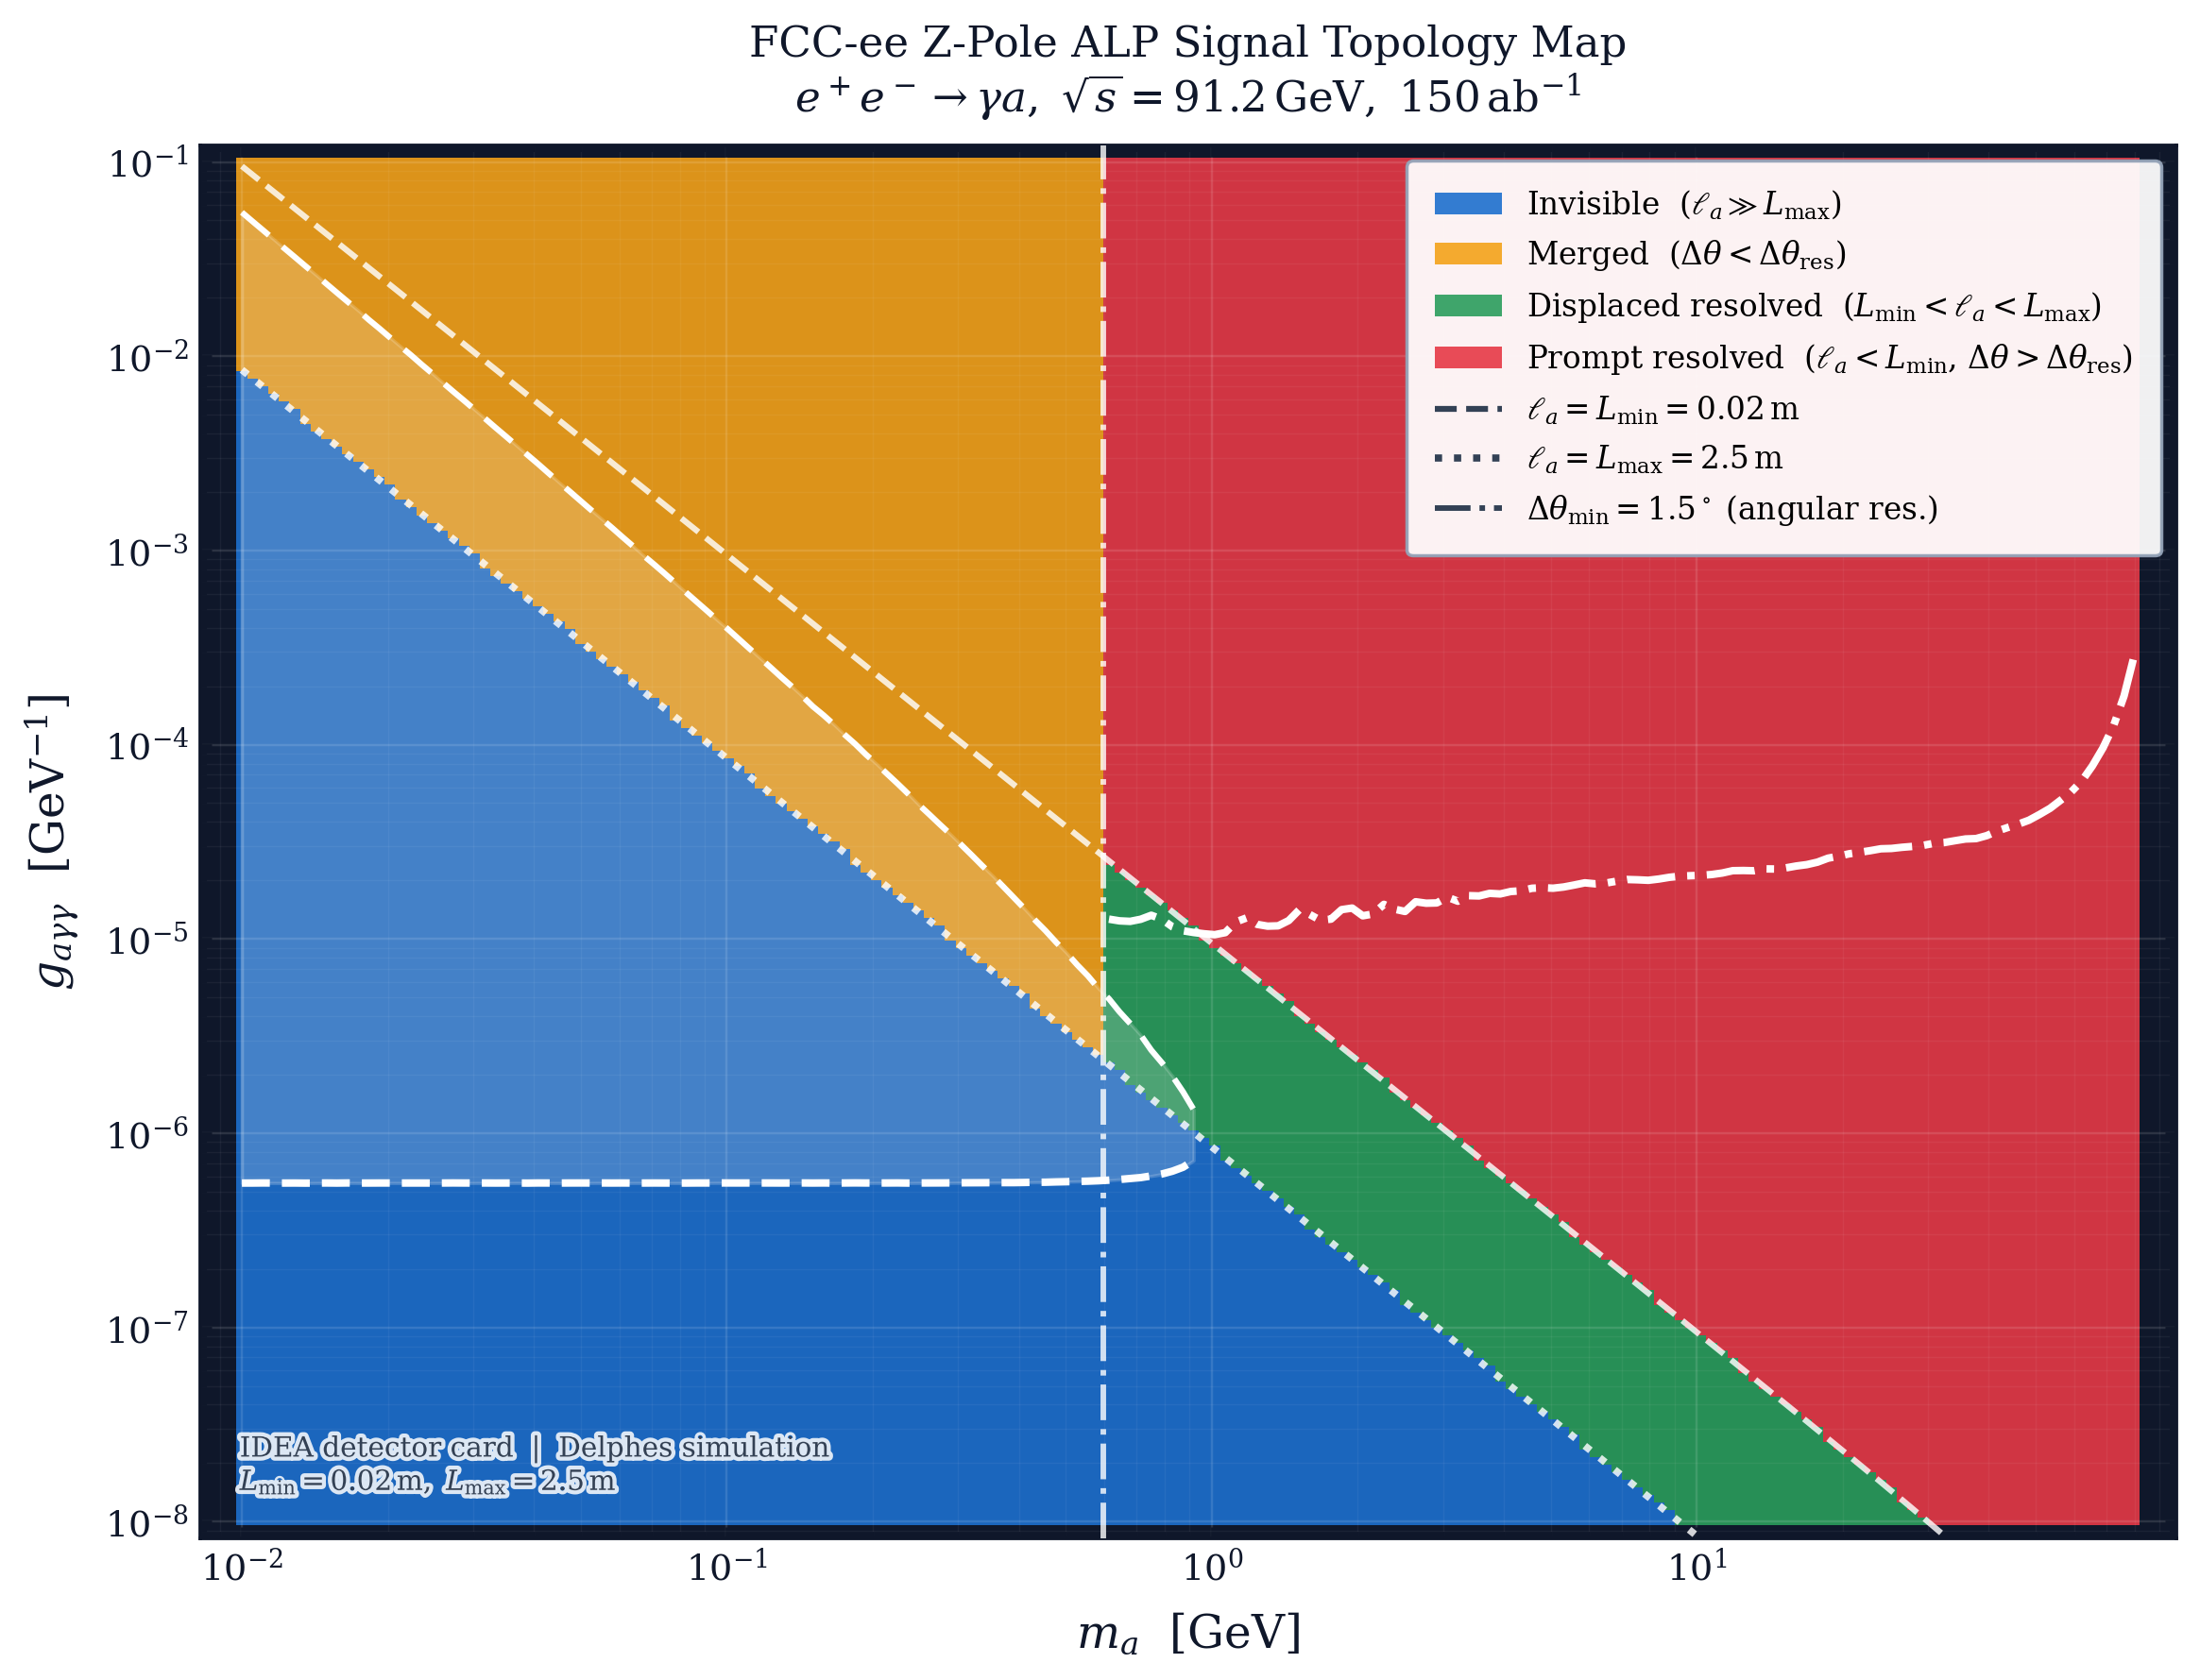
\includegraphics[width=0.75\textwidth]{results/fccee/fccee_zpole_signature_classification.png}
    \caption{ALP signature classification in the $(m_a, g_{a\gamma\gamma})$ plane
    for the FCC-ee Z pole ($\sqrts = 91.2\GeV$) under IDEA detector assumptions.
    Dashed lines show the analytic $\ell_a = L_\mathrm{min}$ (prompt/displaced boundary)
    and $\ell_a = L_\mathrm{max}$ (displaced/invisible boundary) curves.
    The thin dash-dot curve shows the angular-resolution boundary
    $\Delta\theta = \Delta\theta_\mathrm{res} = 1.5^\circ$.
    Only the invisible and prompt-resolved signatures are used in the projected
    exclusion contours.}
    \label{fig:classification}
\end{figure}

\subsection{Projected exclusion contours}

Figure~\ref{fig:money} shows the main result: the projected FCC-ee Z-pole
exclusion contours overlaid on the current ALP-photon constraint landscape
from AxionLimits~\cite{AxionLimits}.

\begin{figure}[h]
    \centering
    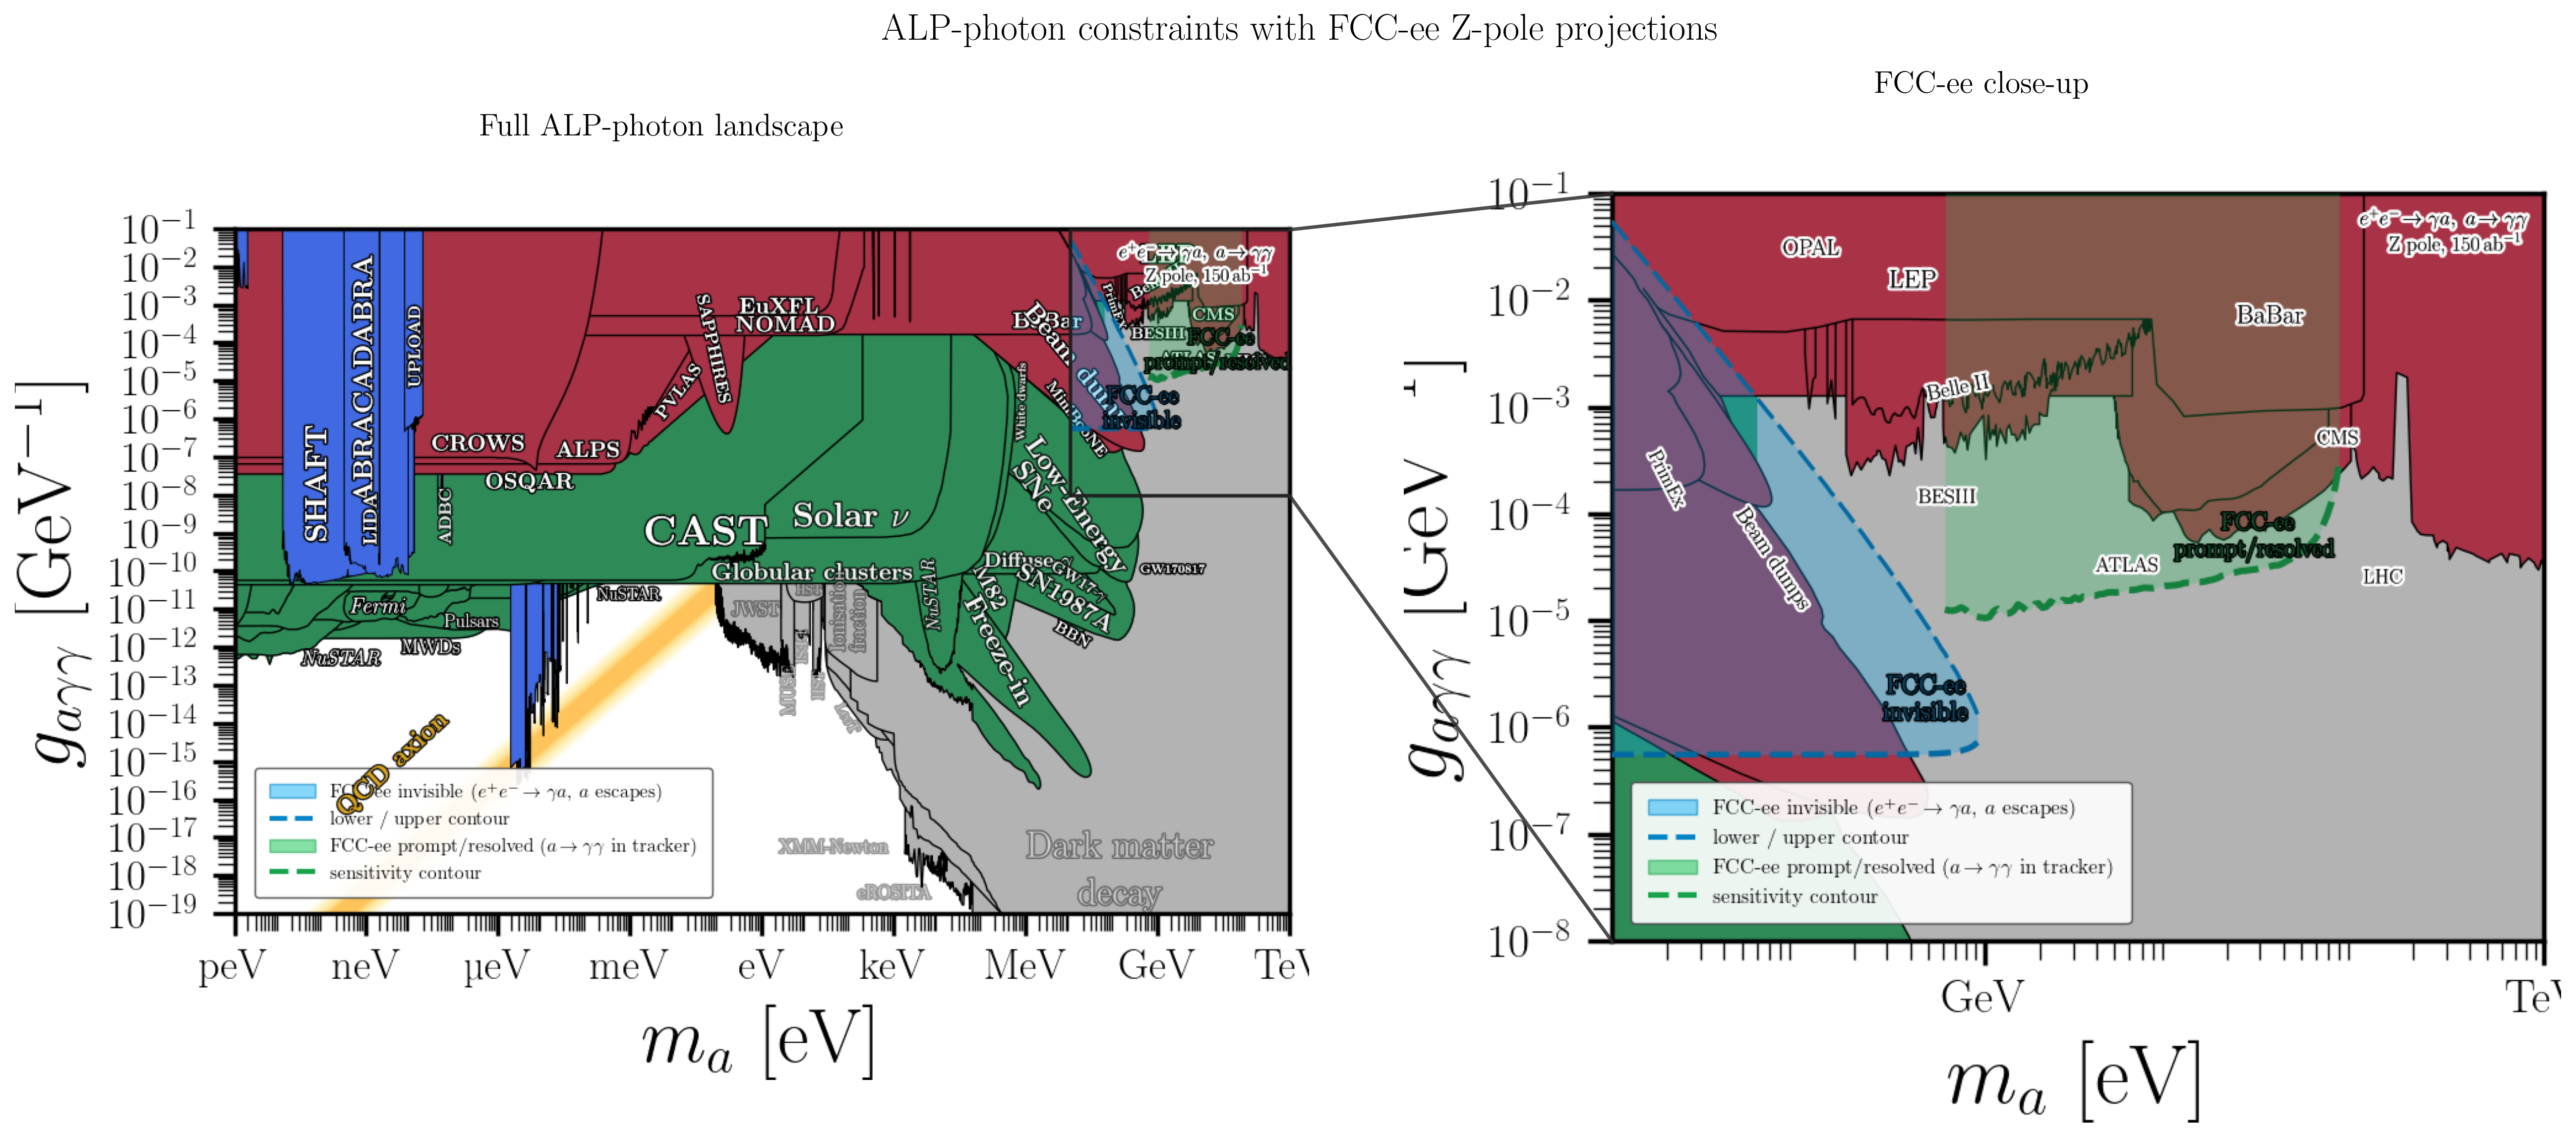
\includegraphics[width=\textwidth]{results/fccee/money_plot_alp_full_combined.png}
    \caption{ALP-photon parameter space with FCC-ee Z-pole projected sensitivity.
    \textit{Left}: full ALP-photon landscape from meV to TeV ALP mass.
    Individual existing constraints are shown as labelled coloured regions
    (stellar/astrophysical in green, helioscope CAST in pink,
    colliders and beam experiments in red/blue tones).
    \textit{Right}: FCC-ee Z-pole zoom region ($10\MeV$--$80\GeV$).
    Shaded blue band: projected invisible exclusion region, bounded below
    (solid dashed line, sensitivity floor) and above (lighter dash, lifetime ceiling).
    Shaded green region: projected prompt-resolved exclusion, bounded by the
    sensitivity contour (green dashed).
    All constraints shown are existing published bounds.
    Background constraints from AxionLimits~\cite{AxionLimits}.}
    \label{fig:money}
\end{figure}

The external regions in Fig.~\ref{fig:money} are used as a landscape, not as a
single statistically homogeneous exclusion. AxionLimits combines direct
laboratory searches, stellar-energy-loss bounds, cosmological arguments, dark
matter-motivated projections, and QCD-axion reference bands. These inputs do
not all share the same assumptions about ALP abundance, branching fractions,
early-universe history, or statistical treatment. The FCC-ee curves overlaid
here are different in character: they are direct collider projections for the
photophilic benchmark of Eqs.~\eqref{eq:lagrangian} and
\eqref{eq:photophilic_split}, with no assumption that the ALP is dark matter
or that it solves the strong CP problem. Regions labelled by cosmology,
stellar physics, and QCD-axion model lines are therefore important context for
the global ALP landscape, but they do not replace the controlled collider
question answered by this repository.

\paragraph{Invisible channel.}
The invisible sensitivity spans $m_\alp \in [0.01, 0.92]\GeV$.
The lower contour (sensitivity floor) sits at:
\begin{equation}
    \gagg^\mathrm{inv} \approx 5.5\times10^{-7}\GeV^{-1}
    \quad(\text{nearly flat across the mass range}),
    \label{eq:inv_result}
\end{equation}
representing a factor $\sim 10$--$100$ improvement over the current best
collider bounds in this mass range.
The near-flatness of the lower contour reflects the dominance of the
signal statistics floor (3 events) over the background shape at high luminosity.
The upper contour rises from $\gagg \approx 1.3\times10^{-6}\GeV^{-1}$ at
$m_\alp = 0.01\GeV$ to $\gagg \approx 0.055\GeV^{-1}$ at $m_\alp = 0.92\GeV$,
marking the transition to the short-lifetime (prompt) regime.

\paragraph{Prompt-resolved channel.}
The prompt-resolved sensitivity spans $m_\alp \in [0.61, 80]\GeV$.
The lower mass threshold is set by Eq.~\eqref{eq:threshold}.
The exclusion contour runs from:
\begin{equation}
    \gagg^\mathrm{res} \in
    \left[1.1\times10^{-5},\; 2.9\times10^{-4}\right]\GeV^{-1}
    \quad \text{(at } m_\alp = 0.61\text{--}80\GeV\text{)}.
    \label{eq:res_result}
\end{equation}
In the mass range $1$--$10\GeV$, the prompt-resolved sensitivity at FCC-ee
extends below the current Belle~II and BaBar limits by roughly one to two orders
of magnitude.

\paragraph{Comparison to existing limits.}
Table~\ref{tab:comparison} summarises the FCC-ee reach at selected masses
compared to the best current bounds.

\begin{table}[h]
    \centering
    \caption{FCC-ee projected sensitivity versus current best limits at representative masses.
    Current limits from AxionLimits~\cite{AxionLimits}.}
    \label{tab:comparison}
    \begin{tabular}{llll}
        \toprule
        $m_\alp$ & Channel & Current best $\gagg$ [$\GeV^{-1}$] &
        FCC-ee projected $\gagg$ [$\GeV^{-1}$] \\
        \midrule
        $0.1\GeV$ & Invisible & $\sim10^{-4}$ (beam dumps) &
        $5.5\times10^{-7}$ \\
        $1\GeV$ & Prompt-resolved & $\sim10^{-3}$ (Belle~II) &
        $\sim3\times10^{-5}$ \\
        $10\GeV$ & Prompt-resolved & $\sim10^{-4}$ (BaBar) &
        $\sim2\times10^{-5}$ \\
        $50\GeV$ & Prompt-resolved & $\sim10^{-3}$ (LEP) &
        $\sim2\times10^{-4}$ \\
        \bottomrule
    \end{tabular}
\end{table}

% ============================================================
\section{Discussion}
\label{sec:discussion}

\subsection{Physics reach}

The FCC-ee Z-pole presents a qualitatively different sensitivity landscape
from any existing experiment.
At low ALP masses ($m_\alp \lesssim 0.1\GeV$), the invisible channel exploits
the huge luminosity to push the sensitivity floor below
$\gagg \sim 10^{-6}\GeV^{-1}$, a regime otherwise accessible only to
stellar observations (HB stars, SN~1987A).
At intermediate masses ($1$--$10\GeV$), the prompt-resolved channel cleanly
covers the region between current $B$-factory limits and LEP.
At high masses ($10$--$80\GeV$), the prompt-resolved channel overlaps with
and significantly improves on LEP and LHC constraints, benefiting from the
clean $e^+e^-$ environment and the mono-energetic photon tag.

The invisible channel's sensitivity has a fundamental lower limit set by
the 3-event floor in Eq.~\eqref{eq:nsig_req}: at exactly 3 required events
and $\Lint = 150\abinv$, the cross section threshold corresponds to
$\sigma_\mathrm{min} = 3 / (1.5\times10^8\,\text{pb}^{-1})
= 2\times10^{-8}\,\text{pb}$.
From Eq.~\eqref{eq:xsec}, this maps to
$\gagg \approx 5\times10^{-7}\GeV^{-1}$, consistent with
Eq.~\eqref{eq:inv_result}.
A nearly background-free invisible analysis at this luminosity would be
statistics-limited. In the implemented binned-background analysis, the
background shape raises the required signal yield above three events for some
masses (for example to about 10.7 events at the lightest masses), but the
result remains driven mainly by the enormous FCC-ee luminosity and the
$\sigma\propto\gagg^2$ scaling.

\subsection{Confidence in the projection}

The results should be interpreted as a detector-corrected phenomenological
projection, not as an experimental limit. Within that scope, the confidence is
highest where the analysis is controlled by validated analytic formulae and
moderate detector corrections, and lower where small lifetime probabilities
are amplified by large correction factors.

\begin{table}[h]
    \centering
    \caption{Reliability assessment of the main ingredients in the projection.}
    \label{tab:confidence}
    \begin{tabular}{p{0.25\textwidth}p{0.18\textwidth}p{0.47\textwidth}}
        \toprule
        Ingredient & Confidence & Reason \\
        \midrule
        Production normalisation &
        High &
        The associated-production cross section is analytic and Gate~1 agrees
        with MadGraph for all 284 detector-level signal points. \\
        Width and lifetime convention &
        High &
        The $64\pi$ width convention is locked in the parameter-card writer,
        Pythia receives the same lifetime, and Gate~2 checks the convention. \\
        Belle~II closure logic &
        High at public-contour level &
        Gate~3 reproduces the digitised Belle~II boundary to a maximum
        residual of $7.6\times10^{-3}$ in $\log_{10}\gagg$. \\
        Prompt-resolved FCC-ee contour &
        Moderate to high &
        The branch has reasonable Delphes correction factors
        (median close to one, range 0.90--2.62) and a direct invariant-mass
        validation at detector level. \\
        Invisible lower contour &
        Moderate to high &
        The lower branch is controlled by production rate, survival
        probability near unity, recoil-energy validation, and correction
        factors close to one. \\
        Invisible upper contour &
        Low to moderate &
        This is a lifetime ceiling where the invisible probability changes
        extremely rapidly with $\gagg$; the detector-correction factors become
        very large in the low-mass tail. \\
        Absolute experimental reach &
        Moderate &
        The study includes leading SM backgrounds and Delphes response, but not
        full detector systematics, machine backgrounds, or a real FCC-ee
        experimental likelihood. \\
        \bottomrule
    \end{tabular}
\end{table}

The most robust headline statements are therefore the existence of strong
FCC-ee reach in the invisible lower branch and in the prompt-resolved branch,
the location of the resolved threshold near $0.6\GeV$, and the qualitative
separation of invisible, prompt/resolved, merged, and displaced regions. The
least robust feature is the precise position of the invisible upper branch,
which should be described as the expected lifetime boundary rather than as a
precision contour.

\subsection{Limitations and caveats}

Several important caveats apply to the current projections.

\paragraph{Invisible upper branch.}
The invisible upper contour (the lifetime ceiling) carries very large detector
correction factors ($C_\mathrm{Delphes} \sim 10^6$--$10^8$ in parts of the
low-mass tail).
These arise because the analytic invisible probability
$P_\mathrm{inv} = e^{-L_\mathrm{max}/\ell_a}$ plunges steeply as $\gagg$
increases, while the Delphes simulation shows a slightly smoother falloff
due to ISR and finite detector response.
The upper branch should be treated as directional rather than precise.

\paragraph{Detector systematics.}
The current analysis includes only the dominant SM backgrounds for each
channel and does not account for:
systematic uncertainties on photon reconstruction efficiency and energy scale;
machine-induced backgrounds from beamstrahlung and synchrotron radiation
(relevant at FCC-ee);
pileup-like machine backgrounds;
and higher-order QED and electroweak corrections to the SM background rates.

\paragraph{Merged and displaced signatures.}
The merged and displaced-resolved signatures together cover 24\% of the
$(m_\alp, \gagg)$ grid.
Merged photons require dedicated cluster-shape reconstruction, and displaced
diphotons require dedicated vertex-level analysis.
Including these channels would extend the claimed reach to couplings
where the ALP is not fully prompt, potentially filling in the gap between the
invisible and prompt-resolved contours.

\paragraph{Single-iteration Delphes correction.}
The branch-aware detector correction factor is derived from signal points
on the first-iteration projected contour, not at the corrected contour
positions.
A second Delphes campaign at the corrected contour points would be needed for a
fully self-consistent result.

\paragraph{Belle~II closure scope.}
The closure test validates the analysis model at published-contour level.
It does not access Belle~II's private likelihood, background spectra,
or efficiency maps, and should not be read as a full reimplementation of
the Belle~II result.

\subsection{Outlook}

Several extensions would strengthen and broaden the analysis.

\textit{Displaced and merged channels.}
Implementing dedicated reconstruction for displaced and merged topologies
would extend the FCC-ee ALP coverage to a nearly complete $(m_\alp, \gagg)$
map from the resolved threshold ($\ma \approx 0.6\GeV$) all the way to the
kinematic endpoint ($\ma \lesssim \sqrts/2 = 45.6\GeV$), including
the intermediate-lifetime region currently left blank.

\textit{Higher-order corrections.}
ISR corrections and NLO QCD/EW effects on the background processes could shift
the background normalisation by $\mathcal{O}(10\%)$, which at this level of
signal sensitivity may become relevant.

\textit{ALP--$Z$ coupling.}
The present analysis considers only the ALP--photon coupling $\gagg$.
ALPs may also couple to the $Z$ boson, modifying both production and
decay at FCC-ee energies~\cite{Brivio2017,Dolan2017}.
In this repository that coupling is cancelled at tree level by
Eq.~\eqref{eq:photophilic_split}. This is why the projection does not use the
potentially resonant $Z\to\gamma a$ enhancement from the
$5\times10^{12}$ Z bosons expected at the FCC-ee Z pole. Including a nonzero
$C_{\gamma Z}$ would enrich the phenomenology, but it would be a different
two-coupling analysis with additional processes such as $Z\to\gamma a$ and
possibly $e^+e^-\to Za$.

\textit{Other FCC-ee run stages.}
FCC-ee will also operate at the WW threshold, HZ threshold, and $t\bar{t}$
threshold.
The WW and HZ stages provide different kinematics and potentially larger
cross sections for ALPs coupling to $W$ bosons or via Higgs loops,
while the higher $\sqrts$ extends the prompt-resolved reach to higher $\ma$.

% ============================================================
\section{Conclusion}
\label{sec:conclusion}

We have computed projected 90\% CL exclusion contours for photophilic ALPs at
the FCC-ee Z-pole ($\sqrts = 91.2\GeV$, $\Lint = 150\abinv$) using a
complete simulation chain from matrix-element generation to fast detector
response.
For the invisible channel, the analysis achieves sensitivity to
$\gagg \approx 5.5\times10^{-7}\GeV^{-1}$ across the mass range
$m_\alp \in [0.01, 0.92]\GeV$, surpassing current collider bounds by one to
two orders of magnitude.
For the prompt-resolved channel, the contour covers
$m_\alp \in [0.61, 80]\GeV$ at $\gagg \sim 10^{-5}$--$3\times10^{-4}\GeV^{-1}$,
significantly exceeding the reach of existing $e^+e^-$ and LHC experiments.

The analysis is validated against the published Belle~II exclusion boundary
to 0.8\%, confirming the consistency of the analytic production model,
lifetime convention, and signal-region logic.
The simulation chain uses MadGraph5, Pythia~8, and a Delphes IDEA card; the
validation suite also checks the MadGraph cross section, the ALP width and
Pythia lifetime, the Delphes output, and the invariant-mass or recoil-energy
observable for every detector-level signal point.
The most robust parts of the result are the invisible lower branch and the
prompt-resolved contour. The invisible upper branch should be interpreted more
qualitatively because it is a rapidly varying lifetime boundary with large
detector-correction factors.

The results establish FCC-ee as an extraordinarily powerful probe of
photophilic ALPs in the $10\MeV$--$80\GeV$ mass range, potentially
surpassing the world-leading sensitivity of stellar and astrophysical
bounds in a controlled collider environment.
Future work should extend the analysis to displaced and merged signatures,
include machine-induced backgrounds and systematic uncertainties, and
incorporate ALP couplings beyond the photon vertex.

% ============================================================
\section*{Acknowledgements}

The author thanks the Nikhef computing cluster for providing the resources
used for the full-statistics Monte Carlo campaigns, and the AxionLimits
repository~\cite{AxionLimits} for the constraint landscape data.

% ============================================================
\bibliographystyle{unsrtnat}
\begin{thebibliography}{99}

\bibitem{Peccei1977}
R.~D.~Peccei and H.~R.~Quinn,
\textit{CP conservation in the presence of pseudoparticles},
Phys.\ Rev.\ Lett.\ \textbf{38}, 1440 (1977).

\bibitem{Weinberg1978}
S.~Weinberg,
\textit{A new light boson?},
Phys.\ Rev.\ Lett.\ \textbf{40}, 223 (1978).

\bibitem{Wilczek1978}
F.~Wilczek,
\textit{Problem of strong P and T invariance in the presence of instantons},
Phys.\ Rev.\ Lett.\ \textbf{40}, 279 (1978).

\bibitem{Jaeckel2010}
J.~Jaeckel and A.~Ringwald,
\textit{The low-energy frontier of particle physics},
Annu.\ Rev.\ Nucl.\ Part.\ Sci.\ \textbf{60}, 405 (2010),
[\href{https://arxiv.org/abs/1002.0329}{arXiv:1002.0329}].

\bibitem{Brivio2017}
I.~Brivio \textit{et al.},
\textit{ALPs effective field theory and collider signatures},
Eur.\ Phys.\ J.\ C \textbf{77}, 572 (2017),
[\href{https://arxiv.org/abs/1701.05379}{arXiv:1701.05379}].

\bibitem{Dolan2017}
M.~J.~Dolan, T.~Erber, F.~Kahlhoefer, and M.~Schmidt-Hoberg,
\textit{Searching for ALPs with LEP, the LHC and a future circular collider},
JHEP \textbf{10}, 079 (2017),
[\href{https://arxiv.org/abs/1709.03453}{arXiv:1709.03453}].

\bibitem{Jaeckel2016}
J.~Jaeckel and M.~Thormaehlen,
\textit{Distinguishing axion models with the axion-photon coupling},
Phys.\ Rev.\ D \textbf{95}, 015010 (2017),
[\href{https://arxiv.org/abs/1612.00034}{arXiv:1612.00034}].

\bibitem{FCCee_CDR}
A.~Abada \textit{et al.}\ (FCC Collaboration),
\textit{FCC-ee: The lepton collider},
Eur.\ Phys.\ J.\ Special Topics \textbf{228}, 261 (2019),
[\href{https://arxiv.org/abs/1905.05078}{arXiv:1905.05078}].

\bibitem{FCC_Physics}
A.~Abada \textit{et al.}\ (FCC Collaboration),
\textit{FCC physics opportunities},
Eur.\ Phys.\ J.\ C \textbf{79}, 474 (2019),
[\href{https://arxiv.org/abs/1905.05078}{arXiv:1905.05078}].

\bibitem{IDEA}
A.~Abada \textit{et al.},
\textit{IDEA: A detector concept for FCC-ee},
Eur.\ Phys.\ J.\ Special Topics \textbf{228}, 1107 (2019).

\bibitem{Belle2}
I.~Adachi \textit{et al.}\ (Belle~II Collaboration),
\textit{Search for axion-like particles produced in $e^+e^-$ collisions at Belle II},
Phys.\ Rev.\ Lett.\ \textbf{130}, 231801 (2023),
[\href{https://arxiv.org/abs/2206.07598}{arXiv:2206.07598}].

\bibitem{AxionLimits}
C.~O'Hare,
\textit{cajohare/AxionLimits: AxionLimits},
Zenodo (2020),
\href{https://doi.org/10.5281/zenodo.3932430}{DOI: 10.5281/zenodo.3932430},
\url{https://cajohare.github.io/AxionLimits/}.

\bibitem{MG5}
J.~Alwall \textit{et al.},
\textit{The automated computation of tree-level and next-to-leading order differential
cross sections, and their matching to parton showers},
JHEP \textbf{07}, 079 (2014),
[\href{https://arxiv.org/abs/1405.0301}{arXiv:1405.0301}].

\bibitem{Pythia8}
T.~Sjöstrand \textit{et al.},
\textit{Introduction to \textsc{Pythia}~8.2},
Comput.\ Phys.\ Commun.\ \textbf{191}, 159 (2015),
[\href{https://arxiv.org/abs/1410.3012}{arXiv:1410.3012}].

\bibitem{Delphes}
J.~de~Favereau \textit{et al.}\ (DELPHES~3 Collaboration),
\textit{DELPHES 3: A modular framework for fast simulation of a generic detector},
JHEP \textbf{02}, 057 (2014),
[\href{https://arxiv.org/abs/1307.6346}{arXiv:1307.6346}].

\bibitem{Cowan2011}
G.~Cowan, K.~Cranmer, E.~Gross, and O.~Vitells,
\textit{Asymptotic formulae for likelihood-based tests of new physics},
Eur.\ Phys.\ J.\ C \textbf{71}, 1554 (2011),
[\href{https://arxiv.org/abs/1007.1727}{arXiv:1007.1727}].

\end{thebibliography}

% ============================================================
\appendix
\section*{Appendix: Contribution Statement}

Iñaki Pardo led the physics study, repository organization, simulation
campaigns, analysis development, validation, plotting, and writing. The project
was developed in collaboration with project partners and with Codex-assisted
implementation and documentation work. External software, models, detector
cards, constraint data, and papers are credited in the repository provenance
report and bibliography.

\end{document}
